\section{Jakość przybliżania funkcji w metodzie rożnicowej}
\begin{frame}{Jakość przybliżania funkcji w metodzie rożnicowej}
	\begin{figure}[h]
			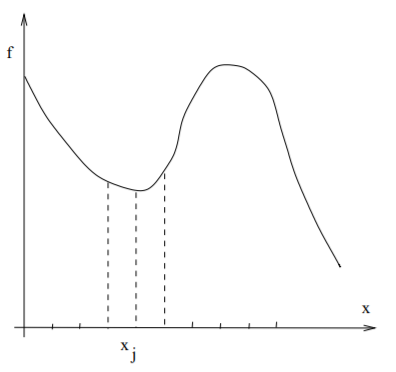
\includegraphics[width=.43\linewidth]{img/20/mrs_img_2}
	\end{figure}
    \begin{exampleblock}{}
    	$\textbf{Dobra:}$ aproksymacja funkcji wolnozmiennej (długofalowej) 
    \end{exampleblock}
    \begin{alertblock}{}
    	$\textbf{Zła:}$ przybliżenie na siatce funkcji szybkozmiennej
    \end{alertblock}
\end{frame}
%%%%%%%%%%%%%%%%%%%%%%%
\begin{frame}
	\begin{figure}[h]
			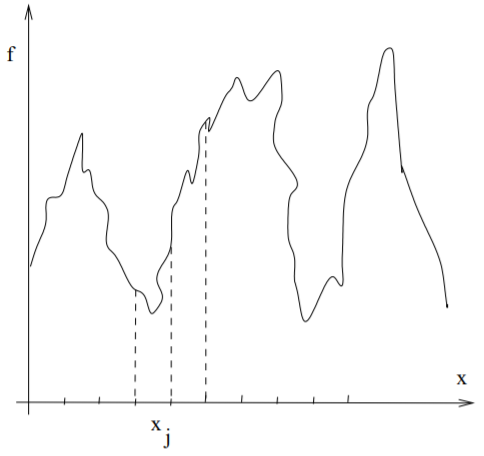
\includegraphics[width=.40\linewidth]{img/20/mrs_img_3}
	\end{figure}
    \newcommand\myeq{\mathrel{\overset{\makebox[0pt]{\mbox{\normalfont\tiny\sffamily (w.Dirichleta)}}}{funkcja}}}
    Opis ilościowy $\rightarrow$ analiza fourierowska:
    $\myeq \ \rightarrow \newline \rightarrow$ ciąg modów Fouriera
    $\newline$f(x):
    \[
    	f(x)=\sum_{l=-\infty}^{\infty}g_{l}\cdot e^{i\cdot k_{l}\cdot x},\
         \ k=\frac{2\pi}{L}\cdot l=k_{0}\cdot l
    \]
    \[
    	g_{l}=\frac{1}{L}\int_{L}dxf(x)e^{-ik_{i}x}
         \ \ 
         \textrm{amplituda fali o długości} \
         \lambda = \frac{L}{l}
    \]
\end{frame}
%%%%%%%%%%%%%%%%%%%%%%%
\begin{frame}
	$\{ f_{j} \}: \ \Delta x =  \Delta$ - stała 
    \[
    	f_{j}=\sum_{l=1}^{J}g_{l}\cdot e^{ik_{l}\cdot x_{j}},\ \ \ k_{l}
        \cdot x_{j}=\frac{2.\pi}{J\cdot \Delta}\cdot l\cdot\Delta
        \cdot j=\frac{2\pi j}{J}
    \]
    \[
    	g_{l}= \frac{1}{L}\sum_{j=1}^{J}f_{j}\cdot e^{ik_{l}\cdot x_{j}} 		\textrm{- amplituda}
    \]
    $\newline$
    Na siatce można opisać tylko skończony zbiór fal, istnieje najmniejsza,
    graniczna długość fali, którą można zdefiniować na siatce:
    $\Delta = \frac{l}{J}$
\end{frame}






